% ARTICLE TEMPLATE
% Santiago Parraguez Cerda
% University of Chile 
% santiago.parraguez@ug.uchile.cl
%
% Version: 0.1 (15/06/2021)
% 
% CREATE DOCUMENT
\documentclass[a4paper, 10pt]{article} 
% Article size A4, 10pt (can be change to 'letterpaper' and any size you want).

% IMPORT CONFIGURATIONS
% ==================================
%      DOCUMENT CONFIGURATIONS
% ==================================

%% ------- GENERAL CONFIGURATION ----------
% Language (for babel)
\newcommand{\defaultlanguage} {english}
% Define default image folder
\newcommand{\defaultimagefolder} {img}
% Default interline distance
\newcommand{\defaultinterline} {1.0}
% Default new paragraph skip
\newcommand{\defaultparskip} {5pt}
% Default paragraph indentation
\newcommand{\defaultparindent} {17pt}
% Space before footnotes
\newcommand{\footnotespace}{15pt}
% Space between footnotes
\newcommand{\footnoteskip}{9pt}

% -------------- PAGE FORMAT --------------
% Portrait page top margin [cm]
\newcommand{\firstpagemargintop} {3.0}  
% Page top margin [cm]
\newcommand{\pagemargintop} {3.0}
% Page bottom margin [cm]
\newcommand{\pagemarginbottom} {2.7} 
% Page left margin [cm]
\newcommand{\pagemarginleft} {2.54}
% Page right margin [cm]
\newcommand{\pagemarginright} {2.54}

% -------------- PORTRAIT -----------------
% Header height of the portrait
\newcommand{\portraitheadheight} {70pt}

% -------------- INDEX --------------------
% Insert index
\newcommand{\showindex} {true}
% Show index of tables and figures
\newcommand{\showindextables} {true}
\newcommand{\showindexfigures} {true}
% Add a dot after numbers
\newcommand{\showdotafternum} {true}
% Skip before each section toc
\newcommand{\beforesecskip} {6pt}
% Skip before each subsection toc
\newcommand{\beforesubsecskip} {4pt}
% Skip before each subsubsection toc
\newcommand{\beforesubsubsecskip} {2pt}

% -------------- REFERENCES ---------------
% Sorting order of the references (nty, nyt, nyvt, anyt, anyvt, ydnt, none)
\newcommand{\biblatexsort} {nty}    
% Cite style (numeric, apa, authoryear, ieee)
\newcommand{\biblatexstyle} {apa}
% Max number of authors in apa configuration
\newcommand{\biblatexmaxapa} {99}
% Space between cite entries [pt]
\newcommand{\bibentrysep} {5pt}

% --------------- FLOAT OBJECTS -----------
% Indicate caption position, only for calculation. This does not mean that the caption is actually placed at top or bottom.
\newcommand{\tablecaptiontop} {true}
\newcommand{\figurecaptiontop} {false}
% Add section number to figures and tables
\newcommand{\fignumsec} {false}
\newcommand{\tabnumsec} {false}
% Figure default placement
\newcommand{\figureplacement}{htb}
% Table default placemente
\newcommand{\tableplacement}{htb}

% -------------- NAME OBJECTS -------------
% \newcommand{\nameabstract} {Abstracter}
\newcommand{\nametablecontents} {Table of Contents}
\newcommand{\namelisttables} {List of Tables}
\newcommand{\namelistfigures} {List of Figures}
\newcommand{\namereferences} {References}
% \newcommand{\namefigure} {Figurechan}
% \newcommand{\nametable} {Tablekun}
% \newcommand{\namesrc} {Source Codehack}
% \newcommand{\nameappendix} {Appendixix}


% IMPORT PACKAGES
% =================
%  PACKAGE IMPORTS
% =================
\usepackage[utf8]{inputenc}

\usepackage{array}
\usepackage{amsmath}
\usepackage{authblk}
\usepackage{booktabs}
\usepackage{caption}
\usepackage{csquotes}
\usepackage{fancyhdr}
\usepackage{geometry}
\usepackage{graphicx}
\usepackage{hyperref}
\usepackage{ifthen}
\usepackage{indentfirst}
\usepackage{lipsum}
\usepackage{microtype}
\usepackage{multirow}
\usepackage{ragged2e}
\usepackage{slantsc}
\usepackage{setspace}
\usepackage{titlesec}
\usepackage{xcolor}

% PACKAGE WITH CONFIGURATIONS
% ---------------------------
\usepackage[english]{babel}
\usepackage[shortlabels]{enumitem}

% CONDITIONAL PACKAGES
% --------------------
% BIBLATEX
\ifthenelse{\equal{\biblatexstyle}{apa}}{
    \usepackage[backend=biber, natbib, style=\biblatexstyle, sorting=\biblatexsort, uniquelist=false, apamaxprtauth=\biblatexmaxapa]{biblatex}
    }{
    \usepackage[backend=biber, natbib, style=\biblatexstyle, sorting=\biblatexsort, uniquelist=false]{biblatex}
}

% IMPORT COMMANDS
% =================
% TEMPLATE COMMANDS
% =================

% DEFINE ABSTRACT AND KEYWORDS
\renewcommand{\abstract}[1]{
    \def\theabstract{#1}
    }
\newcommand{\keywords}[1]{
    \def\thekeywords{#1}
    }
\newcommand{\corrauthor}[1]{
    \def\thecorrauthor{#1}
    }

% MAKETITLE COMMAND
\makeatletter
\renewcommand\maketitle{
    {\raggedright\LARGE\rmfamily\@title\\
    \vspace{0.5em}}
    \large\rmfamily\sffamily\@author\\
    \vspace{.1em} \hrule \vspace{1.2em}
    \normalfont
    \begin{tabular*}{\textwidth}{@{\extracolsep{\fill}} p{0.23\textwidth} @{} p{0.7\textwidth} @{}}
        \large{\textls[150]{\textsc{keywords}}} & \large{\textls[150]{\textsc{abstract}}} \\
        \addlinespace[0.4em]
        \cmidrule{1-1}\cmidrule{2-2}
        \addlinespace[0.25em]
        \raggedright\thekeywords & \theabstract \\
    \end{tabular*}
    \vspace{1.0em} \hrule \vspace{1.0em}
    }
\makeatother

% DEFINE NEW COLUMN TYPES FOR TABULAR
\newcolumntype{L}[1]{>{\raggedright\let\newline\\\arraybackslash\hspace{0pt}}m{#1}}
\newcolumntype{C}[1]{>{\centering\let\newline\\\arraybackslash\hspace{0pt}}m{#1}}
\newcolumntype{R}[1]{>{\raggedleft\let\newline\\\arraybackslash\hspace{0pt}}m{#1}}

% DEFINE TABLENOTE COMMAND
\newcommand{\tablenote}[2][-0.1em]{
    \renewcommand\arraystretch{100}
    \vspace{#1}\\{\footnotesize#2}
    }
    
% DEFINE BLIND FOOTNOTE
\newcommand\blfootnote[1]{%
    \begin{NoHyper}
    \renewcommand{\thefootnote}{}
    \footnotetext{#1}
    \renewcommand{\thefootnote}{\arabic{footnote}}
    \end{NoHyper}
}

% DEFINE PAGESTYLE
\fancypagestyle{core}{
	\fancyhf{}
	\rfoot{\thepage}
	\renewcommand{\headrulewidth}{0pt}
	\renewcommand{\footrulewidth}{0.4pt}
    }

% IMPORT INITIAL CONFIGURATION
% =================
%  DOCUMENT INIT
% =================

% CHANGE DEFAULT IMAGE FOLDER
\graphicspath{{./\defaultimagefolder}}

% Set page margins in cm (requires 'geometry')
\newcommand{\setpagemargincm}[4]{
    \newgeometry{left=#1cm, top=#2cm, right=#3cm, bottom=#4cm}
}

% RENEW AUTHOR AND AFFILIATION CONFIG
\renewcommand\Authfont{\normalfont}
\renewcommand\Affilfont{\slshape\footnotesize}
\renewcommand\Authsep{, }
\renewcommand\Authand{ and }
\renewcommand\Authands{ and }
\setlength{\affilsep}{.8em}

% FORMATTING SECTION TITLES
\titlelabel{\thetitle. }

\titlespacing*{\section}{0pt}{1.2ex plus .5ex minus .2ex}{.6ex plus .2ex}
\titlespacing*{\subsection}{0pt}{1.2ex plus .5ex minus .2ex}{.6ex plus .2ex}
\titlespacing*{\subsubsection}{0pt}{1.2ex plus .5ex minus .2ex}{.6ex plus .2ex}

% SET PARAGRAPH CONFIGURATIONS
\setlength{\parskip}{\setparskip}
\setlength{\parindent}{\setparindent}
\renewcommand{\baselinestretch}{\setbaselinestretch}

% INSERT REFERENCES
\addbibresource{references.bib}
\setlength{\bibhang}{1.5em}
\setlength{\bibitemsep}{.2em}
\renewcommand*{\bibfont}{\normalfont\small}

% CONFIGURE CAPTIONS
\captionsetup[table]{
    labelfont=bf, 
    labelsep=newline, 
    singlelinecheck=false, 
    skip=0.2\baselineskip
    }
\captionsetup[figure]{
    labelfont=bf, 
    singlelinecheck=false, 
    skip=0.4\baselineskip
    }
% \setlength\tabcolsep{0pt}

% SET COLOURS FOR LINKS
\definecolor{urlcolor}{rgb}{0.02, 0.27, 0.68}
\hypersetup{
    colorlinks=true,
    linkcolor=black,
    filecolor=cyan,
    citecolor=black,
    urlcolor=urlcolor
    }

% SET LIST CONFIGURATIONS
\setlist{itemsep=-0.2em}


% ======== DOCUMENT INFORMATION ========
% TITLE
\title{A new study of high scientific impact on a variety of topics}

% AUTHORS
\author[a]{Albert Einstein}
\author[b, c]{Marie Skłodowska}
\author[d]{Isaac Newton}

% AFFILIATIONS
\affil[a]{University of Zürich, Zürich, Switzerland.}
\affil[b]{University of Paris, Paris, France}
\affil[c]{She was the first person to win the Nobel Prize twice, and the only one to win the Nobel Prize in two scientific fields.}
\affil[d]{Trinity College, Cambridge, United Kingdom}

% ABSTRACT
\abstract{
This template allows you to create a well formatted Latex manuscript. You can change the title, authors, affiliations, abstract and keywords easily in the main.tex file. The main document must be written or inserted below "Insert sections", were I will leave a few examples of useful things you can do with this template.
}

% Keywords
\keywords{
\LaTeX, Github, Template, Paper, Open-Source
}

% =======================================
\begin{document}

% PAGE CONFIGURATIONS
% ====================
%  PAGE CONFIGURATION
% ====================

% Set page margins
\setpagemargincm{\pagemarginleft}{\pagemargintop}{\pagemarginright}{\pagemarginbottom}

% Set column separation
\setlength{\columnsep}{\columnseparation}

% SET ABOVE AND BELOW DISPLAY SKIP
\setlength{\abovedisplayskip}{.5em}
\setlength{\belowdisplayskip}{1em}

% Make document two column and add title
\twocolumn[
\maketitle
]

% APPLY PAGE STYLE
\pagestyle{core}

% =======================================
% INSERT SECTIONS (here you can write your document)
% ==============================
\section{Introduction}
% ==============================

This template is based on the article class and supports almost all the functions of that class. Also, in the config.tex file you can find some customisation options that I automated to make the template easier to use. In the following sections I will detail some examples and guides to use the template.
% ==============================
\section{Using the template}
% ==============================

This is a different section. You can write directly to the main.tex file, or write your document to these auxiliary files, it's up to you. You can create multiple new files if you want, it is more convenient for me to have one file for each section.

\subsection{Cite using Biblatex}

The Biblatex package has been loaded into the document, this package provides advanced bibliographic facilities for use with LaTeX. There are multiple ways of loading and use this package, so I recommend to read the documentation for advanced users. Below are shown some of the citation options:

\begin{itemize}
    \item \verb+\cite{Raghavan2007}+ produces \cite{Raghavan2007}
    \item \verb+\citep{Lou2013}+ produces \citep{Lou2013}
    \item \verb+\citeauthor{Newman2004}+ changes if the number of authors is too low: \citeauthor{Newman2004}
    \item \verb+\citeyear{Sobolevsky2014}+ produces \citeyear{Sobolevsky2014}
\end{itemize}

You should consider that the configuration in which the package was loaded will affect what each command prints.

\subsection{Insert figures, tables and equations}

Below are some basic examples for inserting different content into the manuscript. Note that the configuration with which a figure or table is inserted will define where it is located.

\subsubsection{Figures}

An image file is provided, so that you can see an example of image insertion.

\begin{figure}[htb]
    \centering
    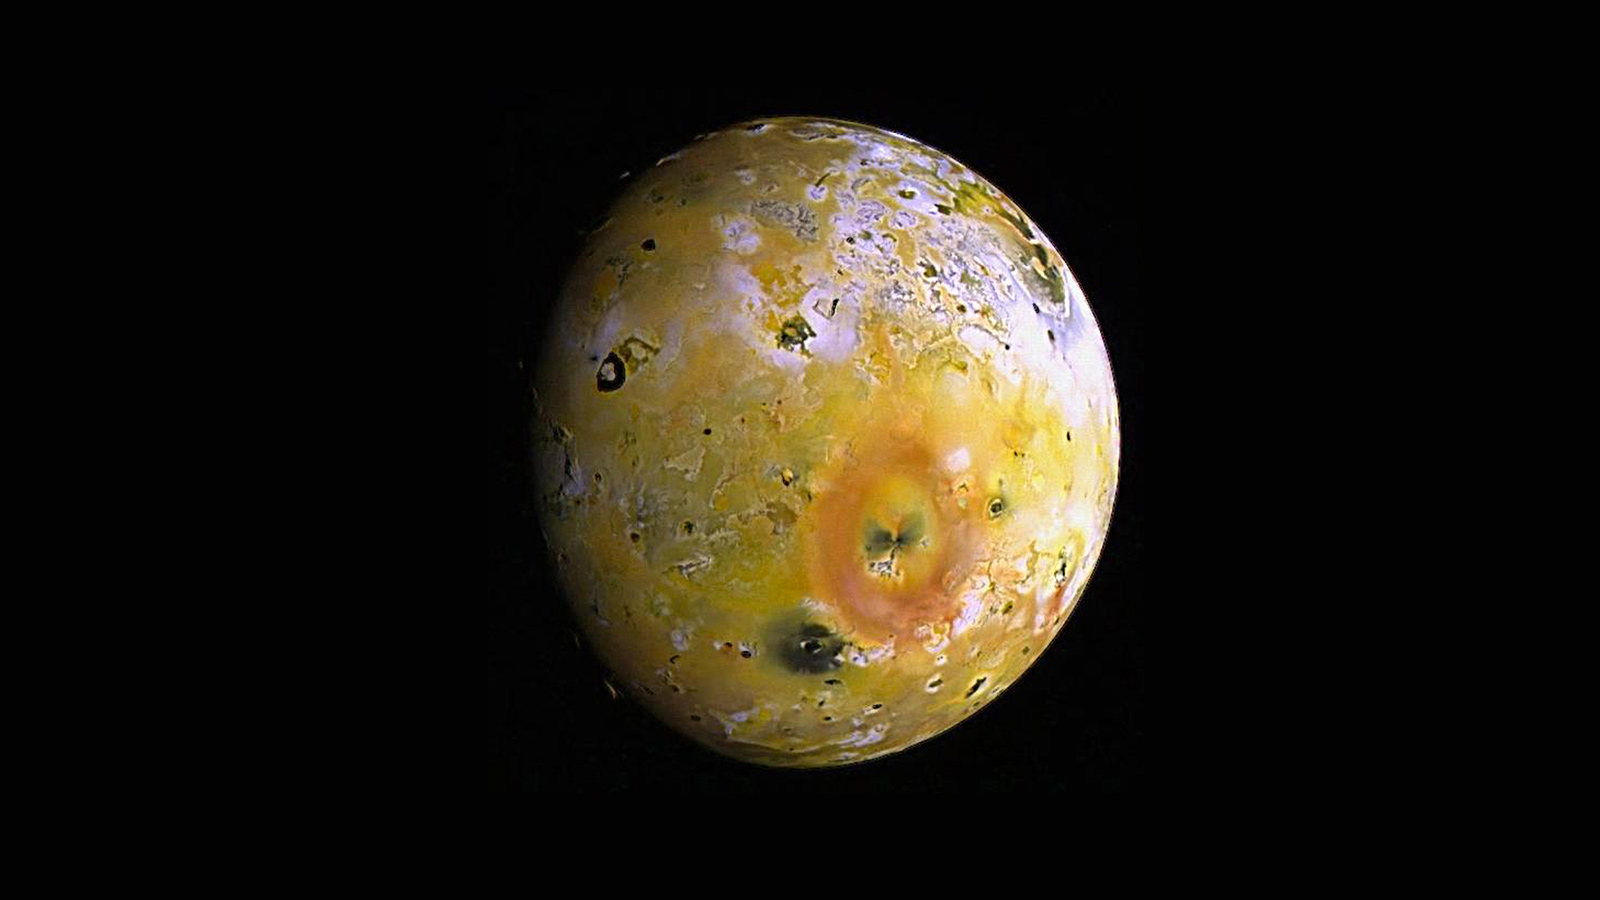
\includegraphics[width=0.8\columnwidth]{img/io_moon.jpg}
    \caption{Io is the innermost and third-largest of the four Galilean moons of the planet Jupiter.}
    \label{fig:my_label}
\end{figure}

If you change the environment into \verb+\begin{figure*}+ \verb+...+ \verb+\end{figure*}+ you will get a single column figure inserted.

\subsubsection{Tables}

There are a variety of ways to insert tables in Latex, so only one way will be exemplified that allows them to look similar to manuscripts.

First of all, we have the Table \ref{tab:population}. This is how a table would be written to use the width of the column and delete the extra space on the sides.

\begin{table}[htb]
    \caption{Countries with the largest population in the world.}
    \label{tab:population}
    \begin{tabular*}{\columnwidth}{@{\extracolsep{\fill}} *{2}{l} r @{}}
        \toprule
        \# & Country & Population (2020) \\
        \midrule
        1 & China & 1,439,323,776 \\
        2 & India & 1,380,004,385 \\
        3 & United States & 331,002,651 \\
        4 & Indonesia & 273,523,615 \\
        5 & Pakistan & 220,892,340 \\
        \bottomrule
    \end{tabular*}
\end{table}

Of course, there are cases where our tables contain too much information, so it is not possible to adapt them to the width of a column. In those cases we can create a table with the width of all the text, as seen in Table \ref{tab:extended_population}. Furthermore, I have defined the \verb+\tablenote+ command to add footnotes to tables.

\begin{table*}[htb]
    \caption{Countries with the largest population, but with more data.}
    \label{tab:extended_population}
    \begin{tabular*}{\textwidth}{@{\extracolsep{\fill}} *{6}{l} @{}}
    \toprule
        \# & Country & Population (2020) & Yearly change & Net change & Density ($n/km^2$)\\
        \midrule
        1 & China & 1,439,323,776 & 0.39\% & 5,540,090 & 153 \\
        2 & India & 1,380,004,385 & 0.99\% & 13,586,631 & 464 \\
        3 & United States & 331,002,651 & 0.59\% & 1,937,734 & 36 \\
        4 & Indonesia & 273,523,615 & 1.07\% & 2,898,047 & 151 \\
        5 & Pakistan & 220,892,340 & 2.00\% & 4,327,022 & 287 \\
        \bottomrule
    \end{tabular*}
    \tablenote{Source: United Nations, Department of Economic and Social Affairs, Population Division. \href{https://esa.un.org/unpd/wpp/}{World Population Prospects: The 2019 Revision.} (Medium-fertility variant).}
\end{table*}

\subsubsection{Equations}

We can easily insert equations using the environment \verb+\begin{equation} ... \end{equation}+. Equations inserted through this environment are automatically numbered. For example we can write the heat equation.

\begin{equation}
    \frac{\partial u}{\partial t} = \alpha \Delta u
\end{equation}

On the other hand we can write this function in Cartesian coordinates, assuming $u(x,y,z,t)$ as solution of the equation.

\begin{equation}
    \frac{\partial u}{\partial t} = \alpha \left( \frac{\partial^2 u}{\partial x^2} + \frac{\partial^2 u}{\partial y^2} + \frac{\partial^2 u}{\partial z^2} \right)
    \label{eq.2}
\end{equation}

You can the reference this equations if you add them a label using \verb+\ref{eq.2}+ and this will gives you the number of the equation (\ref{eq.2}).

% =======================================
\printbibliography
\end{document}
